\documentclass[10pt]{article}
\usepackage[utf8]{inputenc}
\usepackage[T1]{fontenc}
\usepackage{amsmath}
\usepackage{amsfonts}
\usepackage{amssymb}
\usepackage[version=4]{mhchem}
\usepackage{stmaryrd}
\usepackage{graphicx}
\usepackage[export]{adjustbox}
\graphicspath{ {./images/} }

\begin{document}
\section*{Propositional Logic}
The only assignment I that verifies both (2.1) and (2.3) is the one with $I\left(B_{1}\right)= T$ and $I\left(B_{2}\right)=I\left(B_{3}\right)=F$, which implies that the gold is in the first box.

\section*{*}
\section*{Exercise 2.25.}
Kyle, Neal, and Grant find themselves trapped in a dark and cold dungeon (HOW they arrived there is another story). After a quick search the boys find three doors, the first one red, the second one blue, and the third one green.

Behind one of the doors is a path to freedom. Behind the other two doors, however, is an evil fire-breathing dragon. Opening a door to the dragon means almost certain death.

On each door there is an inscription:\\
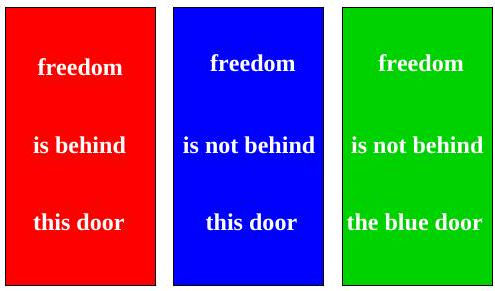
\includegraphics[max width=\textwidth, alt={}, center]{ac6934a9-4003-46d2-9fc8-4f05631a4142-24_291_495_1416_746}

Given the fact that at LEAST ONE of the three statements on the three doors is true and at LEAST ONE of them is false, which door would lead the boys to safety?

\section*{Solution.}
\section*{Language}
\begin{itemize}
  \item $r$ : "freedom is behind the red door"
  \item $b$ : "freedom is behind the blue door"
  \item $g$ : "freedom is behind the green door"
\end{itemize}

\section*{Axioms}
\begin{enumerate}
  \item "behind one of the door is a path to freedom, behind the other two doors is an evil dragon"
\end{enumerate}


\begin{equation*}
(r \wedge \neg b \wedge \neg g) \vee(\neg r \wedge b \wedge \neg g) \vee(\neg r \wedge \neg b \wedge g) \tag{2.4}
\end{equation*}


\begin{enumerate}
  \setcounter{enumi}{1}
  \item "at least one of the three statements is true"
\end{enumerate}


\begin{equation*}
r \vee \neg b \tag{2.5}
\end{equation*}


\begin{enumerate}
  \setcounter{enumi}{2}
  \item "at least one of the three statements is false"
\end{enumerate}


\begin{equation*}
\neg r \vee b \tag{2.6}
\end{equation*}


\section*{Solution}
\begin{center}
\begin{tabular}{|c|c|c||c|c|c|c|}
\hline
$r$ & $b$ & $g$ & 2.5 & 2.6 & 2.5 & $\wedge 2.6$ \\
\hline\hline
$T$ & $F$ & $F$ & $T$ & $F$ & $F$ &  \\
$F$ & $T$ & $F$ & $F$ & $T$ & $F$ &  \\
$F$ & $F$ & $T$ & $T$ & $T$ & $T$ &  \\
\hline
\end{tabular}
\end{center}

Freedom is behind the green door!

\section*{*}
Exercise 2.26.

\section*{The Labyrinth Guardians.}
You are walking in a labyrinth and all of a sudden you find yourself in front of three possible roads: the road on your left is paved with gold, the one in front of you is paved with marble, while the one on your right is made of small stones. Each street is protected by a guardian. You talk to the guardians and this is what they tell you:


\end{document}